% Brief report style paper

% It's about how a somatotopically ordered pattern can be
% re-established in the cortex based on information carried with
% thalamocortical axons afferent from the ventrobasal thalamus, but
% without specifying absolute positions as center-points for the
% barrels. Everything in the paper should be tailored towards arguing
% this idea.

\documentclass[9pt,lineno]{elife}

\usepackage{color}
\usepackage{amsmath,esint}

% Some document-defined commands
\newcommand*\dif{\mathop{}\!\mathrm{d}}
\newcommand{\cmnt}[1]{\textcolor{blue}{#1}}
\newcommand{\dvrg}{\nabla\vcdot\nabla}
\newcommand{\e}{\emph}
\newcommand{\bol}{\textbf}
\newcommand{\mb}[1]{\mathbf{#1}}
\makeatletter
\newcommand*\vcdot{\mathpalette\vcdot@{.35}}
\newcommand*\vcdot@[2]{\mathbin{\vcenter{\hbox{\scalebox{#2}{$\m@th#1\bullet$}}}}}
\newcommand{\code}[1]{\textsf{#1}}

\title{Modelling the emergence of whisker barrels}

\author[1*]{Sebastian~S.~James}
\author[2]{Leah~A.~Krubitzer}
\author[1]{Stuart~P.~Wilson}

\affil[1]{Department of Psychology, The University of Sheffield, Sheffield, United Kingdom.}
\affil[2]{Center for Neuroscience, The University of California, Davis, United States.}
\corr{seb.james@sheffield.ac.uk}{SSJ}

%\keywords{Barrel cortex $|$ Self-organization $|$ Somatotopic map $|$ Axon guidance}

\begin{document}

\maketitle

\begin{abstract}
Brain development relies on an interplay between genetic specification and
self-organization. Striking examples of this relationship can be found in the
somatosensory brainstem, thalamus, and cortex of rats and mice, where the
arrangement of the facial whiskers is preserved in the arrangement of cell
aggregates to form precise somatotopic maps. We show in simulation how
realistic whisker maps can self-organize, by assuming that information is
exchanged between adjacent cells only, under the guidance of gene expression
gradients. The resulting model provides a simple account of how patterns of
gene expression can constrain spontaneous pattern formation to faithfully
reproduce functional maps in subsequent brain structures.
\end{abstract}

\section{Introduction}

Spatial patterns in neural connectivity provide clues about the constraints
under which brains evolve and develop \citep{purves_iterated_1992}. Perhaps
the most distinctive pattern can be found in the barrel cortex of many rodent
species \citep{woolsey_structural_1970}. The barrels are identifiable soon
after birth in layer 4 of primary somatosensory cortex as dense clusters of
thalamocortical axons, which are enclosed by borders a few neurons thick from
postnatal day 3 \citep{erzurumlu_development_2012}. In the plane tangential to
the cortical surface the barrels constitute a somatotopic map of the whiskers,
with cells within adjacent barrels responding most strongly and quickly to
deflection of adjacent whiskers \citep{armstrong-james_flow_1992}. Barrel
patterning reflects subcortical whisker maps comprising cell aggregates called
barrelettes in the brainstem and barreloids in the thalamus
\citep{ma_barrelettesarchitectonic_1991,van_der_loos_barreloids_1976}.

Barrel formation requires afferent input from whisker stimulation and thalamic
calcium waves \citep{anton-bolanos_prenatal_2019}, and depends on a complex
network of axon guidance molecules such as ephrin-A5 and A7 and adhesion
molecules such as cadherin-6 and 8
\citep{vanderhaeghen_mapping_2000,miller_epha7-ephrin-a5_2006}.  This network
is orchestrated by interactions between morphogens Fgf8 and Fgf17 and
transcription factors Emx2, Pax6, Sp8, and Coup-tf1
\citep{shimogori_fibroblast_2005,bishop_regulation_2000}, which are expressed
in gradients that mark orthogonal axes and can be manipulated to stretch,
shrink, shift, and even duplicate barrels
\citep{assimacopoulos_fibroblast_2012}.

The barrel boundaries form a Voronoi tessellation across the cortical sheet
\citep{senft_mouse_1991} (Fig.\,1A), suggesting that barreloid topology is
preserved in the projection of thalamocortical axons into the cortex, and that
a barrel forms by lateral axon branching from an initial center-point that
ceases upon contact with axons branching from adjacent centers.  However, the
assumption of pre-arranged center-points is difficult to resolve with the
observation that axons arrive in the cortical plate as an undifferentiated
bundle, \emph{prior} to barreloid formation \citep{agmon_organized_1993}.

% Note: The key difference between this theory and the chemospecificity theory
% is that of group membership.

Alternatively, reaction-diffusion dynamics could generate a Voronoi
tessellation without pre-arranged centers, by amplifying characteristic modes
in a noisy initial distribution of axon branches, as a net effect of
short-range cooperative and longer-range competitive
interactions. Accordingly, the barrel pattern would be determined by the
relative strength of these interactions and by the shape of the cortical field
boundary. However, intrinsic cortical dynamics alone cannot account for the
topographic correspondence between thalamic and cortical domains, the
irregular sizes and specific arrangement of the barrels in rows and arcs, or
the influence of gene expression gradients.

The center-point and reaction-diffusion models are not mutually
exclusive. Pre-organized centers could bias reaction-diffusion processes to
generate specific arrangements more reliably, and mechanisms of lateral axon
branching may constitute the tension between cooperation and competition
required for self-organization. However, proof that barrel patterning can
emerge from an undifferentiated bundle of axons, based only on local
interactions, would show that a separate stage and/or extrinsic mechanism for
pre-organizing thalamocortical connections need not be assumed. To this end,
we ask whether barrel maps can emerge in a system with reaction-diffusion
dynamics, under the guidance of signalling gradients, and in the absence of
pre-defined centers.


\section{Models}

\cite{karbowski_model_2004} developed a reaction-diffusion style model of how
extrinsic signalling gradients can constrain the emergence of distinct fields
from intrinsic cortical dynamics. Their model defines how the density of
connections $c(x,t)$ and axon branches $a(x,t)$ interact at time $t$, along a
1D anterior-posterior axis $x$, for $N$ thalamocortical projections indexed by
$i$. The model was derived from the assumption that the rates at which $a_i$
and $c_i$ grow are reciprocally coupled. Extending the original 1D model to
simulate arealization on a 2D cortical sheet, we use $a_i(\mb{x},t)$ and
$c_i(\mb{x},t)$, and model synaptogenesis as
%
\begin{equation} \label{eq:dc}
\frac{\partial c_i}{\partial t} =-\alpha c_i +\beta  \left(1 - \sum_{j=1}^{N} c_{j}\right)[a_i]^k.
\end{equation}
%
Accordingly, where the total density of synaptic connections sums to one,
connections decay at rate $\alpha$. Otherwise the connection density increases
non-linearly ($k>1$) with the density of axon branching. Axon branching is
modelled as
%
\begin{equation} \label{eq:da}
\frac{\partial a_i}{\partial t} = \nabla\vcdot\left(D \nabla a_i-a_i\sum_{j=1}^{M} \gamma_{i,j}\nabla \rho_j(\mb{x}) \cmnt{+ \chi_i}\right) - \frac{\partial c_i}{\partial t}.
\end{equation}
%
The first term on the right describes the divergence (indicated by
$\nabla\vcdot$) of the quantity in parentheses, which is referred to as the
`flux' of axonal branching. The flux represents diffusion across the cortical
sheet, at rate $D$, and the influence of $M$ molecular signalling fields,
$\rho(\mb{x})$. The influence of a given field (indexed by $j$) on a given
thalamic projection (indexed by $i$), is determined by $\gamma_{i,j}$, which
may be positive or negative in order that axons may branch in the direction of
either higher or lower concentrations. Note that computing the divergence in
simulation requires cells on the cortical sheet to communicate with immedately
adjacent cells only (see \emph{Materials \& Methods}) The second term on the
right quantifies the coupling between axon branching and synaptogenesis. Here
  $\chi_i=0$ is a placeholder.

\section{Results}

\begin{figure}
\begin{fullwidth}
%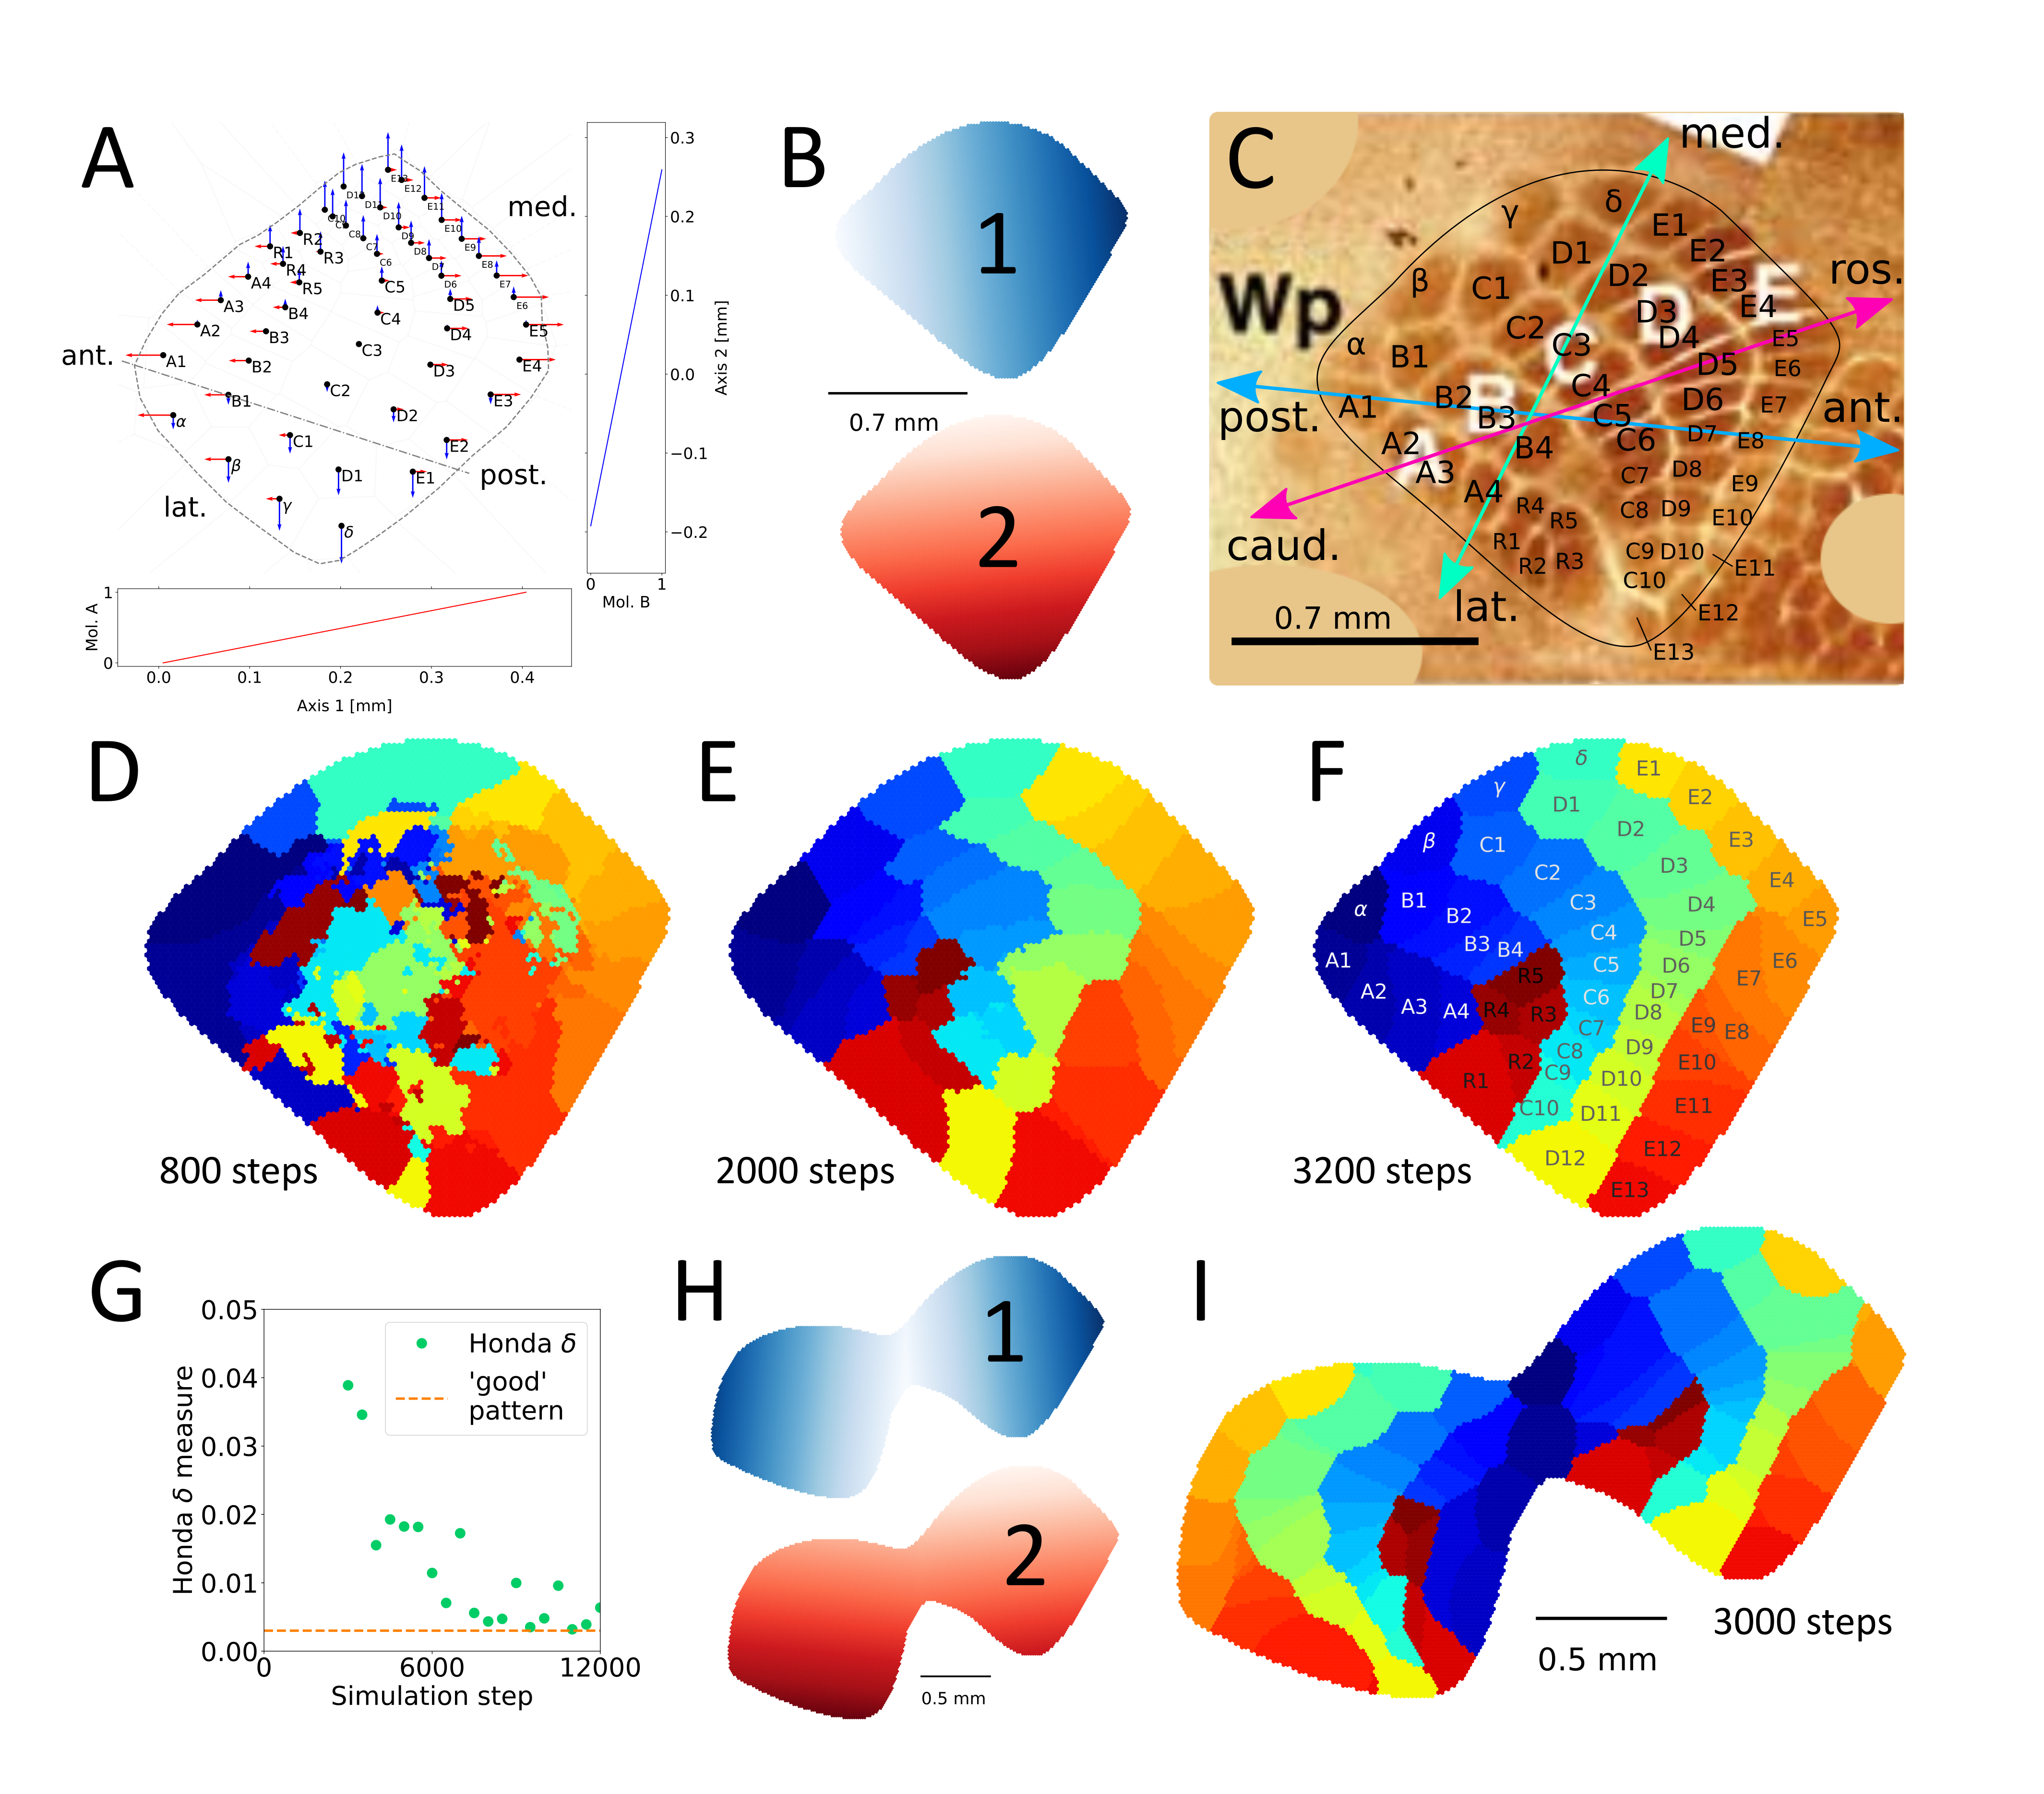
\includegraphics[width=\linewidth]{./MainFig.png}
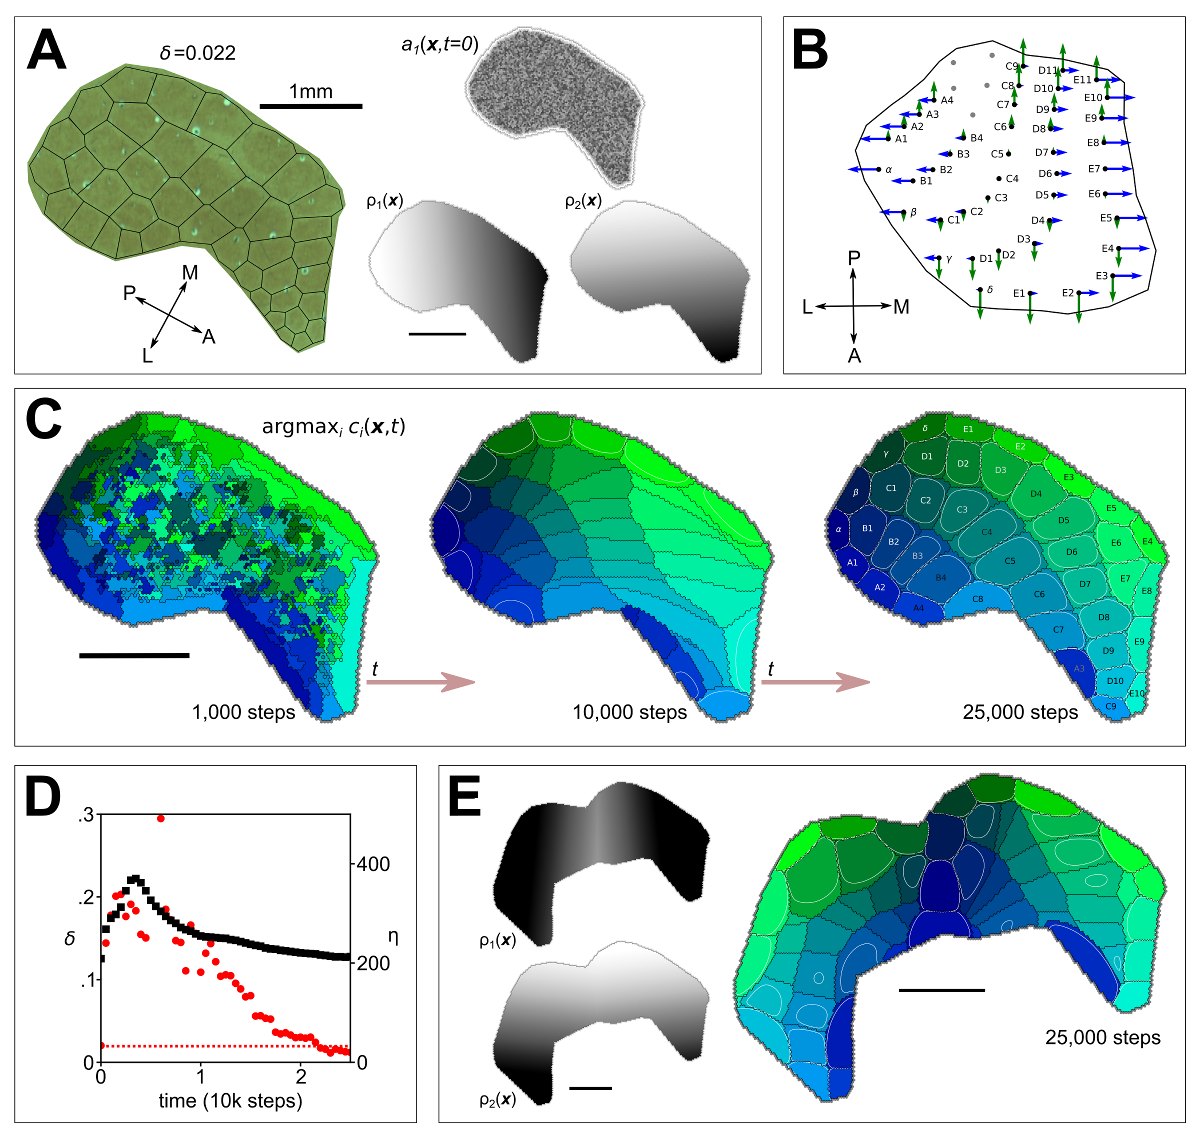
\includegraphics[width=\linewidth]{./MainFig_superlowres.png}
\caption{\textbf{A} Left shows a cytochrome oxidase stain obtained from rat S1
  by \cite{zheng_signal_2001}, with black lines to delineate barrels and to
  measure departure (Honda-$\delta$; see \citealp{senft_mouse_1991}) from a
  perfect Voronoi tesselation. Right shows the initial distribution of axon
  branching density ($a$) for one thalamocortical projection, and two
  molecular guidance fields ($\rho$). \textbf{B} The strengths of interaction
  $\gamma$ with fields $\rho_1$ and $\rho_2$ are indicated for each of 41
  projections by the lengths of green and blue arrows respectively, assuming
  that similar fields aligned to the posterior-anterior and medial-lateral
  axes in the ventroposterior medial nucleus of the thalamus are sampled at
  the locations of putative barreloid centers (reconstructed from
  \citealp{haidarliu_size_2001}). \textbf{C} Simulation results for parameters
  $N=41$, $\alpha=3$, $\beta=20$, $k=3$, $D=0.2$, $\gamma\in\pm 2$,
  $\epsilon=150$ and $\delta{t}=0.0001$. Colours indicate the thalamic
  projection for which the connection density is maximal, black lines
  delineate boundaries, and overlaid contours show $c>0.5$ (see Movie
  S1). \textbf{D} Red dots show the Honda-$\delta$ metric obtained from
  simulation approaching that obtained from barrels in \textbf{A} (dotted
  line); black squares measure the correspondence between the real and
  simulated barrel shapes, $\eta$ (the product of the sum of squared
  differences between real and simulated centers and the sum of differences in
  area; units mm$^4$). \textbf{E} Guidance fields and emergent barrel pattern
  in a Fgf8 misexpression experiment
  (c.f. \citealp{assimacopoulos_fibroblast_2012}), simulated by reflecting
  $\rho_1$ at the join ($\epsilon=80$). All scale bars 1mm.}
\label{fig:main}
\end{fullwidth}
\end{figure}

First we verified that all results established by \cite{karbowski_model_2004}
for a 1D axis could be reproduced using our extension to a 2D cortical
sheet. Using an elliptical domain, $S$, with $M=3$ offset guidance gradients
aligned to the longer axis, $N=5$ thalamocortical projections gave rise to
five distinct cortical fields at locations that preserved the topographic
ordering defined by the original $\gamma$ values. However, we found that
specifying $N$ ordered areas required $M\approx (N+1)/2$ signalling
fields. This is because localization of axon densities occurs only when
projections are influenced by interactions with two or more signalling
gradients that encourage migration in opposing directions. Note that these
dynamics are quite unlike classic chemospecificity models
\citep{sperry_chemoaffinity_1963}, which essentially assume center-points
i.e., conditions in the target tissue that instruct pre-identified afferents
to stop growing. As the number of distinct guidance fields is unlikely to
approach the number of barrels, further extensions were required.

The term in parentheses in Eq.\,\ref{eq:dc} represents competition between
thalamocortical projections for a limited availability of cortical
connections. To introduce competition also in terms of axon branching we
% EITHER
%%redefined
%%%
%%\begin{equation} \label{eq:comp}
%%\color{blue}
%%\chi_i(\mb{x}, t) = \frac{\bar{a}_i F}{N-1} \nabla \sum_{j\ne i}{a_j}
%%\color{black}
%%\end{equation}
% OR
\cmnt{first define a quantity to represent the branching density of all
  \emph{other} TC types; $\hat{a}_i = \sum_{j\ne i}{a_j}$; then set the term
  $\chi_i$ to be}
%
\begin{equation} \label{eq:comp}
\color{blue}
\chi_i(\mb{x}, t) = \frac{\bar{a}_i F}{N-1} \nabla \hat{a}_i
\color{black}
\end{equation}

%
\cmnt{where $F$ is a parameter and $\bar{a}_i$ is a bounded version of $a_i$
  obtained by passing the branching density through the sigmoid function}
%
\begin{equation} \label{eq:abar}
\color{blue}
  \bar{a}_i = \frac{2}{1+\mathrm{e}^{5 - 0.5 a_i}}.
\color{black}
\end{equation}
%
\cmnt{In this expression for $\bar{a}_i$ (only), we model the idea
 that there must be an upper bound on the axonal branching density.}

\cmnt{which contributes to the \emph{flux of axonal branching} by making branching
  density for each projection `flow away' from regions} where the branches of
other projections are dense. Note that this operation is local to individual
afferent projections.

The only differences between thalamic projections are their strengths of
interaction with the guidance fields, $\gamma$, hence any reliable differences
between emergent cortical fields must be due to differences in these values
only. We speculate that the contribution of a given ephrin field, to the
velocity at which a projection migrates across the cortical subplate, is
determined by the concentration of a similar molecule at its thalamic origin,
i.e., the putative barreloid center. As such, two orthogonal linear thalamic
gradients were defined, from which 41 pairs of $\gamma$ values were sampled,
at the coordinates of 41 barreloid centers recreated from
\cite{haidarliu_size_2001} (Fig.\,1B).

A cortical boundary enclosing 41 corresponding barrels was traced from a
cytochrome oxidase stain from \cite{zheng_signal_2001}, and
Eqs.~\ref{eq:dc}--\ref{eq:norm} were solved for $N=41$ projections on the
resulting domain, using $M=2$ linear signalling gradients aligned with the
anterior-posterior and medial-lateral axes. From random initial conditions for
$a(\mb{x},0)$ and $c(\mb{x},0)$, a clear Voronoi-like tesselation emerged
(Fig.\,1C; see Movie S1). A reduction in the Honda delta metric (see
\citealp{senft_mouse_1991}) confirmed that a `good' Voronoi pattern emerged
within $\approx 3000$ iterations (Fig.\,1D). A measure of the difference
in shape between real and simulated barrels revealed a strong correspondence
(see Fig.\,1D).

To further investigate the interplay of genetic and intrinsic mechanisms we
simulated a seminal barrel duplication experiment
\citep{shimogori_fibroblast_2005}, first by solving on a cortical domain
comprising two separate, identically shaped cortical boundaries. In this case
one distinct cortical field per thalamic projection emerged, within one of the
two boundaries only, i.e., no duplication. However, merging the two fields to
create an extended mirror-symmetric boundary shape, with an anterior-posterior
guidance field reflected at the join, gave rise to two mirror-symmetrical
barrel fields comprising 2N barrels, i.e., two cortical fields for each
thalamic projection (Fig.\,1E). Together these results suggest that by the
misexpression of Fgf8, \cite{shimogori_fibroblast_2005}
effectively created one large barrel field rather than two distinct cortical
fields.

\section{Discussion}

The present results suggest that the key requirements for the emergence of
realistic barrel patterning are i) at each cortical location thalamocortical
projections compete for a limited number of available synaptic connections
(Eqs.~\ref{eq:dc}--\ref{eq:da}), ii) at each location the branching rate of a
given projection is reduced by the density of other projections
(Eq.\,\ref{eq:comp}), and iii) the branch density of each projection is
conserved over time (Eq.\,\ref{eq:norm}).

The emergence of barrels in simulation required competition between thalamic
projections in terms of synaptic connectivity and also competition in terms of
cortical space, as represented by $\chi$, with an implicit requirement for a
self/other identifier amoungst projections. This latter form of competition may
account for the absence of barrels in rodents with larger brains, such as
capybara, for which competition for space is presumably weaker
\citep{woolsey_comparative_1975}. Hence, irrespective of whether barrels are
necessary for adaptive whisker function, the emergence of somatotopically
ordered modular structures may be an inevitable consequence of local
competition for cortical territory driven by input from an array of discrete
sensory organs \citep{purves_iterated_1992}.

It is important to emphasize that the formulation of the model is entirely
local, insofar as simulation requires no information to be communicated from a
given cortical grid cell to any but those immediately adjacent (via
diffusion). Hence the simulations demonstrate how a self-organizing system,
constrained by genetically specified guidance cues and by the shape of the
cortical field boundary, can faithfully reproduce an arrangement of cell
aggregates in one neural structure as a topographic map in another.

Moreover, the present results confirm that somatotopic map formation does not
require the pre-specification of center-points by as yet undetermined
additional developmental mechanisms.

\section{Materials \& Methods}

% Be sure to include/mention:
%
% The no-flux boundary conditions applied in the \cite{karbowski_model_2004}
% model are retained.
%
% Arbitrary boundary shapes were applied

The cortical sheet was modelled as a two dimensional hexagonal lattice, which
simplifies the computation of the 2D Laplacian. Within a boundary traced
around the edge of a
rat barrel field (Fig.\,1A) we set the hex-to-hex distance
$d$ to 0.03\,mm, which resulted in a lattice containing 6515 hexes for the
simulations shown in Figs.\,1A,C \& D and 12739 hexes for the Fgf8
misexpression study shown in Fig.\,1E. Each hex contained 82 time-dependent
variables: 41 branching densities ($a_i$) and 41 connection densities ($c_i$).
The rate of change of each of the time-dependent variables (Eqs.\,\ref{eq:dc}
\& \ref{eq:da}) was computed using a fourth-order Runge-Kutta method.

The most involved part of this computation is to find the divergence of the
flux of axonal branching, $\mb{J}_i(\mb{x},t)$, the term in parentheses in
Eq.\,\ref{eq:da}:
%
\begin{equation}
  \label{eq:divJ}
  \nabla\vcdot\mb{J}_i(\mb{x},t) = \nabla\vcdot\left(D \nabla a_i-a_i\sum_{j=1}^{M} \gamma_{i,j}\nabla \rho_j(\mb{x})\right).
\end{equation}
%
Note that the sum of the guidance gradients is time-independent and define
$\mb{g}_i(\mb{x}) \equiv \sum_{j=1}^{M} \gamma_{i,j} \nabla\rho_j(\mb{x})$.
Because the divergence operator is distributive, Eq.\,\ref{eq:divJ} can be
expanded using vector calculus identities (dropping references to $\mb{x}$ and
$t$ for clarity):
%
\begin{equation}
\nabla\vcdot\mb{J}_i = \nabla\vcdot\big(D \nabla a_i\big) - \nabla\vcdot\big(a_i \mb{g}_i\big).
\end{equation}
%
Applying the vector calculus product rule identity yields
%
\begin{equation} \label{eq:divJExpanded}
%
\nabla\vcdot\mb{J}_i =
%
D \dvrg a_i % term1
-
a_i\nabla\vcdot\mb{g}_i % term2
-
\mb{g}_i\vcdot\nabla a_i % term3
,
\end{equation}
%
which has three elements to compute: i)~$D \dvrg a_i$ (the Laplacian of
$a_i$); ii)~a time-independent modulator of $a_i$ (because
$\nabla\vcdot\mb{g}_i$ is a time-independent static field); and iii)~the
scalar product of the static vector field $\mb{g}_i$ and the gradient of
$a_i$. Each of the divergences can be simplified by means of Gauss's Theorem
following \cite{lee_hexagonal_2014}.

(i) The computation of the mean value of the Laplacian across one hexagon of
area $\Omega = \frac{\sqrt{3}}{2}d^2$, located at position $\mb{p}_0$, with
neighbours at positions $\mb{p}_1$--$\mb{p}_6$ is
%
\begin{equation} \label{eq:lapl}
\begin{split}
\langle D \dvrg a_i(\mb{p}_0,t) \rangle  = \frac{1}{\Omega} \oiint_\Omega \dvrg a_i(\mb{x}, t) \dif\Omega & = \frac{1}{\Omega} \oint \frac{\partial a_i}{\partial \hat{\mb{n}}} \dif\gamma \\
& \approx \frac{1}{\Omega} \sum_{j=1}^6 \frac{\partial a_i(\mb{p}_j)}{\partial \hat{\mb{n}}} \bigg\rvert_{\mathrm{mid}} v \\
& = \frac{2}{\sqrt{3} d^2} \sum_{j=1}^6 \frac{a_i(\mb{p}_j) - a_i(\mb{p}_0)}{d} \frac{d}{\sqrt{3}} \\
& = \frac{2}{3 d^2} \sum_{j=1}^6 \big(a_i(\mb{p}_j) - a_i(\mb{p}_0)\big),
\end{split}
\end{equation}
%
where $v = d/\sqrt{3}$ is the length of each edge of the hexagon and $\dif\gamma$
is an infinitesimally small distance along its perimeter.

ii) The computation of the second term in Eq.\,\ref{eq:divJExpanded},
$\langle a_i(\mb{p}_0,t)\nabla\vcdot\mb{g}_i(\mb{p}_0)\rangle$, can be written out similarly:

\begin{equation} \label{eq:divg}
\begin{split}
%
\frac{1}{\Omega} \oiint_\Omega a_i\nabla\vcdot\mb{g}_i\;\dif\Omega & = \frac{a_i(\mb{p}_0,t)}{\Omega}  \oint \mb{g}_i\vcdot \dif\hat{\mathbf{n}} \\
%
& \approx \frac{a_i(\mb{p}_0,t)}{\Omega} \sum_{j=1}^{6} \frac{\mb{g}_i(\mb{p}_j) + \mb{g}_i(\mb{p}_0)}{2}\vcdot \hat{\mb{n}}\;v \\
%
& = \frac{2 a_i(\mb{p}_0,t)v}{\sqrt{3}d^2} \sum_{j=1}^{6} \bigg[ \frac{g_i^x(\mb{p}_j) + g_i^x(\mb{p}_0)}{2} \vcdot  \hat{\mb{n}} + \frac{g_i^y(\mb{p}_j) + g_i^y(\mb{p}_0)}{2} \vcdot  \hat{\mb{n}} \bigg] \\
%
%%& = \frac{2 a_i(\mb{p}_0,t)d}{\sqrt{3}d^2\sqrt{3}} \bigg( \sum_{j=1}^{6} \frac{\mb{g}_j^x + \mb{g}_0^x}{2} \vcdot  \hat{\mb{n}} + \sum_{j=1}^{6} \frac{\mb{g}_j^y + \mb{g}_0^y}{2} \vcdot  \hat{\mb{n}} \bigg) \\
%
%\Rightarrow \langle a_i(\mb{p}_0,t)\nabla\vcdot\mb{g}(\mb{p}_0)\rangle &
%\approx \frac{a_i(\mb{p}_0,t)}{3d} \bigg( \sum_{j=1}^{6} \big(g_i^x(\mb{p}_j)
%+ g_i^x(\mb{p}_0)\big) \cos \big(\frac{\pi}{3}(j-1)\big) + \sum_{j=1}^{6}
%\big({g_i^y(\mb{p}_j) + g_i^y(\mb{p}_0)}\big) \sin
%\big(\frac{\pi}{3}(j-1)\big) \bigg), \\
%% Condensing into a single sum:
\Rightarrow \langle a_i(\mb{p}_0,t)\nabla\vcdot\mb{g}(\mb{p}_0)\rangle & \approx \frac{a_i(\mb{p}_0,t)}{3d} \sum_{j=1}^{6} \bigg[ \big(g_i^x(\mb{p}_j) + g_i^x(\mb{p}_0)\big) \cos \big(\frac{\pi}{3}(j-1)\big) + \big({g_i^y(\mb{p}_j) + g_i^y(\mb{p}_0)}\big) \sin \big(\frac{\pi}{3}(j-1)\big) \bigg], \\
%
\end{split}
\end{equation}
%
where $g_i^x$ and $g_i^y$ are the Cartesian components of $\mb{g}_i$. Both this
last expression, and the final expression of Eq.\,\ref{eq:lapl} can
be computed locally, by summing over values of the nearest neighbours.

iii) The final term in Eq.\,\ref{eq:divJExpanded} is the scalar product of two
vector fields which is straightforward to compute from their Cartesian
components.

By separating the computation of Eq.\,\ref{eq:divJ} into parts (i), (ii) \&
(iii), the no-flux boundary condition,
$\mb{J}_i(\mb{x},t)\big\rvert_{\mathrm{boundary}} = 0$, can be fulfilled. On
the boundary, the contribution to $\mb{J}$ resulting from the first term of
Eq.\,\ref{eq:divJExpanded} can be fixed to 0 by the `ghost cell method' in
which, during the evaluation of (i), a hex outside the boundary containing the
same value as the hex inside the boundary is imagined to exist such that the
flux of $\mb{J}$ across the boundary is 0. Then, $\mb{g}_i(\mb{x})$ can be
tailored so that it, and its normal derivative approach 0 at the boundary,
ensuring that the second and third terms of Eq.\,\ref{eq:divJExpanded} also
contribute nothing to $\mb{J}$. This is achieved by applying to
$\mb{g}_i(\mb{x})$ a sharp logistic function of the distance from $\mb{x}$ to
the boundary.

All code required to reproduce these results is available at
\url{https://github.com/ABRG-Models/BarrelEmerge/tree/eLife}. The
computations described in (i), (ii) and (iii) may be found in the class method
\code{RD\_James::compute\_divJ()} which calculates \code{term1}, \code{term2}
and \code{term3}, respectively.

\section{Movie S1 caption}

Movie corresponding to Fig.\,1C in the main paper. Simulation parameters were
$N=41$, $\alpha=3$, $\beta=20$, $k=3$, $D=0.2$, $\gamma\in\pm 2$,
$\epsilon=150$ and $\delta{t}=0.0001$. Colours indicate the thalamic
projection for which the connection density is maximal, black lines delineate
boundaries, and overlaid contours show $c>0.5$. The final frame in the movie
is step 25,000 of the simulation.

\section{Acknowledgments}

The authors thank Jason Berwick at the University of Sheffield for advice and
for access to the rat barrel stains used to construct Fig.\,1A. This work was
supported by a Collaborative Activity Award, \emph{Cortical Plasticity Within
  and Across Lifetimes}, from the James S.~McDonnell Foundation (grant
220020516).

\bibliography{../BarrelEmerge}

\end{document}
